\chapter{Matrix Exponential Methods}\label{ch:matrixEXPMethods}
The primary method for solving the MSR depletion equation is accomplished by transforming it into a system of first order ODEs. This Chapter presents a method called  matrix exponential methods by the author. It is called by this name because it requires the computation of the exponential of a matrix in order to solve the system of ODEs.

Many methods exist for solving systems of first order differential equations. In vector matrix form, the problem involves solving a system of ordinary differential equations of the form,

\begin{equation}
    \frac{d\boldsymbol{y}}{dt} = \boldsymbol{f}(t,\boldsymbol{y}), \quad \boldsymbol{y}({t_{0})} = \boldsymbol{y_{0}}
    \label{eq:ODE_matrix_form}
\end{equation}{}

\noindent
where $\boldsymbol{y}$, $\boldsymbol{f}(t,\boldsymbol{y})$ and $\boldsymbol{y}_{0}$ are column vectors and $\boldsymbol{f}(t,\boldsymbol{y})$ can contain linear and nonlinear terms. 

$$
\boldsymbol{y}(t) = 
\begin{bmatrix}
y_{1}(t) \\
y_{2}(t) \\
\vdots \\
y_{m}(t) \\
\end{bmatrix}, \quad 
\boldsymbol{f}(t,\boldsymbol{y}) = 
\begin{bmatrix}
f_{1}(t, y_{1}, y_{2}, \dots y_{m}) \\ 
f_{2}(t, y_{1}, y_{2}, \dots y_{m}) \\ 
\vdots \\
f_{m}(t, y_{1}, y_{2}, \dots y_{m}) \\ 
\end{bmatrix}, \quad
\boldsymbol{y}_{0} = 
\begin{bmatrix}
y_{1,0} \\
y_{2,0} \\
\vdots \\ 
y_{m,0} \\
\end{bmatrix}
$$

There are many popular methods to solve these equations including Euler, Runge–Kutta and multistep. These methods involve dividing the time domain into discrete lengths and stepping through the domain by approximating each time step from the previous steps solution and a slope between the points. When the function vector $\boldsymbol{f}(t,\boldsymbol{y})$ contains terms that are stiff, these methods become computationally expensive and inaccurate for larger time steps \cite{ash2009} \cite{ODECh82011}.

A more advantageous method for solving Equation \ref{eq:ODE_matrix_form} is the use of exponential time differencing  \cite{ash2009} \cite{cox2002} \cite{bratsos2019}. To explain this method, Equation \ref{eq:ODE_matrix_form} is rewritten in a form that decomposes $\boldsymbol{f}(t,\boldsymbol{y})$ into two operators, one representing a constant linear operator and one for the nonlinear operator. Equation \ref{eq:ODE_matrix_linear_nonlinear_form} shows this separation with $\boldsymbol{L}$ being the linear operator and $\boldsymbol{N}$ being the nonlinear.


\begin{equation}
    \frac{d\boldsymbol{y}}{dt} = \boldsymbol{Ly} + \boldsymbol{N}(t,\boldsymbol{y}) 
    \label{eq:ODE_matrix_linear_nonlinear_form}
\end{equation}{}

Solving Equation \ref{eq:ODE_matrix_linear_nonlinear_form} using a class of methods involving matrix exponentials can  be broken down into two main categories, integration factor and exponential time differencing. Both of the previously stated methods are discussed further in the next sections. 

\section{Integrating Factor Method}
The integrating factor method begins by defining the following expression \cite{Kassam2005},

\begin{equation}
    \boldsymbol{v} = e^{-\boldsymbol{L}t}\boldsymbol{y},
    \label{eq:v_deff_IF_method}
\end{equation}{}

\noindent
where $e^{-\boldsymbol{L}t}$ is the integrating factor. Next, Equation \ref{eq:v_deff_IF_method} is differentiated with respect with time to give,

\begin{equation}
    \frac{d\boldsymbol{v}}{dt} = -e^{-\boldsymbol{L}t}\boldsymbol{L}\boldsymbol{y} + e^{-\boldsymbol{L}t} \frac{d\boldsymbol{y}}{dt}.
\end{equation}{}

\noindent
Multiplying Equation \ref{eq:ODE_matrix_linear_nonlinear_form} by the integrating factor and bringing the linear operator to the right hand side gives, 

\begin{equation}
    e^{-\boldsymbol{L}t}\frac{d\boldsymbol{y}}{dt} - e^{-\boldsymbol{L}t}\boldsymbol{L}\boldsymbol{y} = e^{-\boldsymbol{L}t}\boldsymbol{N}(t,\boldsymbol{y}) = \frac{d\boldsymbol{v}}{dt}.
\end{equation}{}

\noindent
This brings the final form of the equation to solve, 

\begin{equation}
    \frac{d\boldsymbol{v}}{dt} = e^{-\boldsymbol{L}t}\boldsymbol{N}(t,e^{\boldsymbol{L}t}\boldsymbol{v}), 
\end{equation}{}

\noindent
or, 

\begin{equation}
    \frac{d\boldsymbol{v}}{dt} = \boldsymbol{f}(t,\boldsymbol{v}).
    \label{eq:IFM_transformed_equation_to_solve}
\end{equation}{}

Solving Equation \ref{eq:IFM_transformed_equation_to_solve} can be done using any usual Runge–Kutta, or multistep method. For example, the fourth order Runge-Kutta method gives the following formula \cite{Kassam2005}.


\begin{equation}
\begin{split}
    & k_{1} = h\boldsymbol{f}(t_{n},\boldsymbol{v}_{n}) \\
    & k_{2} = h\boldsymbol{f}(t_{n}+h/2, \boldsymbol{v}_{n} + k_{1}/2) \\
    & k_{3} = h\boldsymbol{f}(t_{n}+h/2, \boldsymbol{v}_{n} + k_{2}/2) \\
    & k_{4} = h\boldsymbol{f}(t_{n}+h, \boldsymbol{v}_{n} + k_{3}) \\
    & \boldsymbol{v}_{n+1} \approx \boldsymbol{v}_{n} + \frac{1}{6}(k_{1} + 2k_{2} + 2k_{3} + k_{4}) \\
    & \boldsymbol{y}_{n+1} = e^{\boldsymbol{L} (t_{n}+h)}\boldsymbol{v}_{n+1}
\end{split}
\end{equation}{}

Integrating factor methods have the property of being exact when $\boldsymbol{N}(t,\boldsymbol{y}) = 0$ \cite{ash2009}. 

\section{Exponential Time Differencing}
Exponential time differencing (EDT) methods are very similar to the integrating factor method except for how it handles the nonlinear portion of Equation \ref{eq:ODE_matrix_linear_nonlinear_form}. Deriving the exponential time differencing formula begins by multiplying Equation \ref{eq:ODE_matrix_linear_nonlinear_form} by the integrating factor,

\begin{equation}
    e^{-\boldsymbol{L}t}\bigg( \frac{d\boldsymbol{y}}{dt}-\boldsymbol{L}y\bigg) = e^{-\boldsymbol{L}t}\boldsymbol{N}(t,\boldsymbol{y}),
\end{equation}

\noindent using the product rule this can be written as,

\begin{equation}
    \frac{d}{dt}\bigg(e^{-\boldsymbol{L}t}\boldsymbol{y}\bigg) = e^{-\boldsymbol{L}t}\boldsymbol{N}(t,\boldsymbol{y}).
\end{equation}

\noindent Next the function is integrated from a point $t_{n}$ to $t_{n} + \Delta t$ where $\Delta t = t_{n+1} - t_{n}$,

\begin{equation}
    e^{-(t_{n} + \Delta t)\boldsymbol{L}}\boldsymbol{y}(t_{n} + \Delta t) - e^{-t_{n}\boldsymbol{L}}\boldsymbol{y}(t_{n}) = \int_{t_{n}}^{t_{n}+\Delta t}e^{-\boldsymbol{L}t}\boldsymbol{N}(t,\boldsymbol{y})dt.
\end{equation}

\noindent Let $t = t_{n} + \tau \quad dt = d\tau \quad  \tau \in [0,\Delta t]$, applying these change of variables gives \cite{bratsos2015}, 

\begin{equation}
    e^{-(t_{n} + \Delta t)\boldsymbol{L}}\boldsymbol{y}(t_{n} + \Delta t) - e^{-t_{n}\boldsymbol{L}}\boldsymbol{y}(t_{n}) = \int_{0}^{\Delta t}e^{-\boldsymbol{L}(t_{n} + \tau)}\boldsymbol{N}(t_{n} + \tau,\boldsymbol{y}(t_{n} + \tau))d\tau.
    \label{eq:transformedExpTimeDifferencing}
\end{equation}

\noindent Because $t_{n}$,  $\tau$ and $\Delta t$ are scalars, the exponential can be written as,

\begin{equation}
\begin{split}
     & e^{-\boldsymbol{L}(t_{n}+\tau)} = e^{-\boldsymbol{L}t_{n}}e^{-\boldsymbol{L}\tau} \\ 
     & e^{-(t_{n}+\Delta t)\boldsymbol{L}} = e^{-\boldsymbol{L}t_{n}}e^{-\boldsymbol{L}\Delta t}.
\end{split}
\end{equation}

\noindent Applying to Equation \ref{eq:transformedExpTimeDifferencing}, $e^{\boldsymbol{L}t_{n}}$ cancels out on both sides. This leads to,

\begin{equation}
    e^{-\Delta t\boldsymbol{L}}\boldsymbol{y}(t_{n} + \Delta t) - \boldsymbol{y}(t_{n}) = \int_{0}^{\Delta t}e^{-\boldsymbol{L}\tau}\boldsymbol{N}(t_{n} + \tau,\boldsymbol{y}(t_{n} + \tau))d\tau, 
\end{equation}



\noindent moving $\boldsymbol{y}(t_{n})$ to the right hand side and multiplying both sides by $e^{\Delta t \boldsymbol{L}}$ gives the final result,

\begin{equation}
    \boldsymbol{y}(t_{n} + \Delta t) = e^{\Delta t\boldsymbol{L}}\boldsymbol{y}(t_{n}) + e^{\Delta t\boldsymbol{L}}\int_{0}^{\Delta t}e^{-\boldsymbol{L}\tau}\boldsymbol{N}(t_{n} + \tau,\boldsymbol{y}(t_{n} + \tau))d\tau,
    \label{eq:ETDMethodExact}
\end{equation}

\noindent where $\boldsymbol{L}$ is called the transition matrix.
This formalization is exact and exponential time differencing methods work to approximate the integral of the nonlinear portion. Exponential  time  differencing  methods have the property of being exact when $\boldsymbol{N}(\boldsymbol{y},t) = \text{constant}$ \cite{ash2009}.

Evaluating the integral in Equation \ref{eq:ETDMethodExact} can be done using traditional multistep methods or with Runge-Kutta methods \cite{cox2002}. For example, a fourth order Runge-Kutta approximation for the integral gives the following formula for Equation \ref{eq:ETDMethodExact} \cite{cox2002},

\begin{equation}
\begin{split}
    % an
     \boldsymbol{a}_{n} &= e^{\boldsymbol{L}\Delta t/2}\boldsymbol{y}(t_{n}) + \boldsymbol{L}^{-1}\big(e^{\boldsymbol{L}\Delta t/2} - \boldsymbol{I} \big)\boldsymbol{N}(t_{n},\boldsymbol{y}(t_{n})) \\
    % bn 
    \boldsymbol{b}_{n} &= e^{\boldsymbol{L}\Delta t/2}\boldsymbol{y}(t_{n}) + \boldsymbol{L}^{-1}\big(e^{\boldsymbol{L}\Delta t/2} - \boldsymbol{I} \big)\boldsymbol{N}(t_{n}+\Delta t/2,\boldsymbol{a}_{n}) \\
    % cn
     \boldsymbol{c}_{n} &= e^{\boldsymbol{L}\Delta t/2}\boldsymbol{a}_{n} + \boldsymbol{L}^{-1}\big(e^{\boldsymbol{L}\Delta t/2} - \boldsymbol{I} \big)\big(2\boldsymbol{N}(t_{n}+\Delta t/2,\boldsymbol{b} _{n}) - \boldsymbol{N}(t_{n},\boldsymbol{y}(t_{n}))\big) \\
     % yn
     \boldsymbol{y}(t_{n+1}) &= e^{\boldsymbol{L}\Delta t}\boldsymbol{y}(t_{n}) + \Delta t^{-2}\boldsymbol{L}^{-3}\big([-4\boldsymbol{I} - \Delta t\boldsymbol{L} + e^{\boldsymbol{L}\Delta t}(4\boldsymbol{I} -3\Delta t\boldsymbol{L} + (\Delta t\boldsymbol{L})^{2})]\boldsymbol{N}(t_{n}, \boldsymbol{y}(t_{n}))) \\
     &+ 2[2\boldsymbol{I} + \Delta t\boldsymbol{L} + e^{\boldsymbol{L}\Delta t}(-2\boldsymbol{I} + \Delta t\boldsymbol{L})](\boldsymbol{N}(t_{n} + \Delta t/2, \boldsymbol{a}_{n}) + \boldsymbol{N}(t_{n} + \Delta t/2, \boldsymbol{b}_{n})) \\
     &+ [-4\boldsymbol{I} - 3\Delta t\boldsymbol{L} - (\Delta\boldsymbol{L})^{2} + e^{\boldsymbol{L}\Delta t}(4\boldsymbol{I} - \Delta t\boldsymbol{L})]\boldsymbol{N}(t_{n}+\Delta t, \boldsymbol{c}_{n})\big)
\end{split}
\end{equation}

\section{Stability of the Transition Matrix in Linear Systems}
Particular situations arise in systems for which Equation \ref{eq:ODE_matrix_linear_nonlinear_form} becomes linear when $\boldsymbol{N}(t,\boldsymbol{y}) = 0$. In this scenario, the system becomes:

\begin{equation}
    \frac{d\boldsymbol{y}}{dt} = \boldsymbol{L}\boldsymbol{y}.
\end{equation}

The existence of the solution to the initial value problem $\boldsymbol{y}(t_{0}) = \boldsymbol{y}_{0}$ is guaranteed if the coefficients of $\boldsymbol{L}$ are continuous on a common interval $I$ that contains the point $t_{0}$ \cite{zill2012}. The stability of this problem can be accessed by examining the eigenvalues of the linear operator $\boldsymbol{L}$. 

\section{Solutions to the Matrix Exponential}
When obtaining solutions based on exponential time differencing, an exponential of a matrix needs to be computed. There are multiple computational methods for solving for the matrix exponential, many of them are developed specifically to evaluate $e^{\boldsymbol{A}t}$ or $e^{\boldsymbol{A}t}\boldsymbol{v}$. One evaluates the matrix exponential directly and the other calculates the action of the exponential on a vector. Because of the way in which the linear systems operate in EDT methods,  only the action of the matrix on the vector is required. However, in some of the methods that will be presented only direct evaluation of the matrix exponential is possible. 

Computation of the exponential of a matrix is by far the most difficult part of EDT methods. Not only is the basis for many of the methods mathematically in depth, but they are difficult to deploy on a level that makes the computation of the matrix exponential both fast and accurate. Numerous methods for computing the matrix exponential are discussed here however, they are not limited to the ones presented in this work. 

%%%%%%%%%%%%%%%%%%%%
%% Taylor and Pade 
%%%%%%%%%%%%%%%%%%%%
\subsection{Series Approximations Near the Origin} \label{subsec:seriesapprox}
Solvers of this nature often exploit the following relation when computing the matrix exponential:

\begin{equation}
    e^{\boldsymbol{A}t} = \big(e^{\boldsymbol{A}t/m}\big)^{m},
\end{equation}

\noindent where $m$ is a scalar that \textit{scales} matrix $\boldsymbol{A}t$. This method is known as scaling and squaring. The reason this is done is to reduce the norm of matrix $\boldsymbol{A}t$, especially in situations for $\boldsymbol{A}t$ when $t \rightarrow \infty$ as previously mentioned. For series methods near the origin, the accuracy of the method diminishes as the matrix norm increases. 


\subsubsection{Taylor Series Expansion}
Formally,  matrix exponential is defined using an infinite Taylor series \cite{exokit} \cite{moler2003} \cite{pusa2010}. 
\begin{equation}
    e^{\boldsymbol{A}} = \sum_{k = 0}^{\infty}\frac{1}{k!}\boldsymbol{A}^{k}
    \label{eq:power_series_exp}
\end{equation}

\noindent Therefore, a straight forward way to calculate the matrix exponential is using its formal definition. This method however, is not commonly used in application for either the matrix or the scalar case. The number of terms required to achieve convergence can be large and produce computational inefficiency. This method also suffers from numerical round off errors and from cancellation for large values of $k$ \cite{moler2003}. There is one method in libowski based off of this method. While not commonly used in practice an algorithm for computing the action of the matrix exponential of matrix $\boldsymbol{A} \in \mathbb{C}^{n\times n}$ on matrix $\boldsymbol{B} \in \mathbb{C}^{n\times n_{0}}$ where $n_{0} << n$ was developed by Al-Mohy and Higham based on a truncated Taylor series \cite{higham2011}:

\begin{equation}
    e^{\boldsymbol{A}}\boldsymbol{B} = (e^{2^{-s}\boldsymbol{A}})^{2^{s}}\boldsymbol{B} \approx T_{m}(2^{-s}\boldsymbol{A})^{2^{s}}\boldsymbol{B},
\end{equation}

\noindent where $T_{m}$ is a truncated Taylor series of order $m$. Unlike the other matrix exponential algorithms that will be presented, the Taylor series does not require linear solves. This method was developed using a backward error analysis based on $||\boldsymbol{A}^{k}||^{1/k}$, keeping in mind the computational cost. To reduce the norm of $\boldsymbol{A}$, the Taylor method uses two key preprocessing steps. These steps include shifting and optional balancing. 


\subsubsection{Pad\'e Approximation}
The Pad\'e approximation represents a function by expanding it as a ratio of two power series. A ($p,q$) Pad\'e approximation for $e^{\boldsymbol{A}t}$ is defined by \cite{moler2003}:

\begin{equation}
    e^{\boldsymbol{A}t} \approx R_{p,q}(\boldsymbol{A}t) = \frac{N_{p,q}(\boldsymbol{A}t)}{D_{p,q}(\boldsymbol{A}t)}
    \label{eq:padeApprox}
\end{equation}

\noindent where

\begin{equation}
    N_{p,q}(\boldsymbol{A}t) = \sum_{j=0}^{p}\frac{(p + q - j)!p!}{(p + q)!j!(p - j)!}(\boldsymbol{A}t)^{j},
\end{equation}

\begin{equation}
    D_{p,q}(\boldsymbol{A}t) = \sum_{j=0}^{q}\frac{(p + q - j)!q!}{(p + q)!j!(q - j)!}(-\boldsymbol{A}t)^{j}.
\end{equation}

Pad\'e methods are similar to Taylor series as they approximate a function using a series solution, however, Pad\'e series usually out perform Taylor series. Series solutions methods, such as Pad\'e are also more accurate near the origin, meaning that the matrix norm $||\boldsymbol{A}t||$ must be sufficiently small for the approximation to be accurate \cite{pusa2010}. Yet another problem arises when $\boldsymbol{A}$ has a wide spread of eigenvalues, causing an ill-conditioned linear system  \cite{exokit} \cite{moler2003}. 

There are many ways to develop an algorithm for computing the matrix exponential using the Pad\'e approximation \cite{exokit} \cite{higham2005} \cite{higham2009}. The key in deriving an algorithm is in both understanding the error associated with the size of the matrix norm and limiting the computation time. Moler and Van Loan derived an elegant and simple proof for determining values for $p$, $q$ and $m$ given a matrix norm \cite{moler2003}. As noted by Higham \cite{higham2005}, this derivation contained weaknesses. Moler and Van Loan assumed that the matrix norm needed to be less than one half ($||\boldsymbol{A}t|| < 1/2$) but Higham proved that this was not the case. Higham further showed that the required minimal matrix norm is different for each order of the Pad\'e implementation. Above this norm, a higher order Pad\'e approximation would be required, or matrix scaling would need to take place. One other weakness was the derivation of their error bound. It was designed to be easily computable, which resulted in their error bound not being sharp \cite{higham2005}. When the error bound is not sharp, then it is possible to overscale the matrix, resulting in a loss of accuracy. Higham and Al-Mohy. described two algorithms to resolve the overscaling problem found in Ref. (\cite{higham2005}) and  Ref. (\cite{higham2009}). Reference (\cite{higham2009}) is an updated algorithm to the one described in Ref. (\cite{higham2005}), which works to fix the overscaling problem.


The Pad\'e approximation in combination with scaling and squaring is probably the most widely used method for computing the exponential of a matrix. In fact, the $expm$ function in MATLAB is based on this approach \cite{higham2009}. Two methods based on the Pad\'e approach are implemented in libowski, \textit{Pad\'e - Method 1} and \textit{Pad\'e - Method 2}. Both algorithms work to form a Pad\'e approximation of type $p = q$ and will further be denoted by $m$, combined with scaling and squaring:

\begin{equation}
    e^{\boldsymbol{A}} = (e^{2^{-s}\boldsymbol{A}})^{2^{s}} \approx r_{m}(2^{-s}\boldsymbol{A})^{2^{s}},
\end{equation}

\noindent where $s$ is the scaling and squaring parameter and $\boldsymbol{A}$ is $\boldsymbol{A}t$. The scaling parameter $s$ is chosen to that the exponential is computed with a backward error bounded by the unit roundoff.  Method - 1 is based on the algorithm developed by Higham in Ref. (\cite{higham2005}), in which he backwards error is based on $||\boldsymbol{A}||$. Method - 2 is based on Ref. (\cite{higham2009}) which worked to reduce the problem of over scaling in the Method - 1 by tightening the backwards error based on $||\boldsymbol{A}^{k}||^{1/k}$ where:

\begin{equation}
    ||\boldsymbol{A}^{k}||^{1/k} \leq ||\boldsymbol{A}||, \quad k = 1:\infty.
\end{equation}


\subsection{Solutions Based on the Cauchy Integral Formula}
This method is based on transforming the matrix exponential into the complex plane using the Cauchy integral formula.  The matrix exponential becomes,

\begin{equation}
	e^{\boldsymbol{A}} = \frac{1}{2\pi i}\int_{\Gamma} e^{z}(z\boldsymbol{I} - \boldsymbol{A})^{-1}dz,
	\label{eq:cauchyExp}
\end{equation}

\noindent where $\boldsymbol{A}$ is analytic inside the closed contour $\Gamma$ that winds once around the eigenvalues of $\boldsymbol{A}$ \cite{pusaThesis} \cite{pusa2011} \cite{Trefethen2006}. In practice, it is often required to evaluate the action of the matrix exponential on vector $\boldsymbol{v}$, this leads to evaluating,

\begin{equation}
	e^{\boldsymbol{A}}\boldsymbol{v} = \frac{1}{2\pi i}\int_{\Gamma} e^{z}(z\boldsymbol{I} - \boldsymbol{A})^{-1}\boldsymbol{v}dz.
	\label{eq:cauchyExpVector}
\end{equation}

\noindent When evaluating Equations \ref{eq:cauchyExp} or \ref{eq:cauchyExpVector} it is vital to select a contour that encloses the spectrum of $\boldsymbol{A}t$. If this is not done, then the approximation is inaccurate. There are a number of ways to solve Equations \ref{eq:cauchyExp} or \ref{eq:cauchyExpVector} which involve knowing the nature of the spectrum of the transition matrix $\boldsymbol{A}t$. 


\subsubsection{Rational Approximation}
A more generalized method for evaluating the contour integral can be accomplished by choosing an analytic function $\phi(\theta)$ that maps the real line onto the contour. Because the function $e^{\phi(\theta)}$ decreases exponentially as $|\theta| \rightarrow \infty$ the approximation can be truncated to a finite number of quadrature points. When the spectrum of the transition matrix falls on the left hand side of the complex plane close to the real axis then the contour $\Gamma$ denotes a Hankel like contour that winds from $-\infty-0i$ on the lower half-plane and $\infty+0i$ on the upper half-plane. \cite{Trefethen2006}. This allows for the definition of a general contour function that will enclose the eigenvalues on the left hand side of the complex plane around the negative real axis. 

The idea is to solve the contour integral of the form,

\begin{equation}
    I = \frac{1}{2\pi i}\int_{-\infty}^{\infty}e^{\phi(\theta)}f(\phi(\theta))\phi'(\theta)d\theta.
    \label{eq:generalContourIntegral}
\end{equation}

\noindent The trapezoidal approximation with $N$ points to Equation \ref{eq:generalContourIntegral} becomes,

\begin{equation}
    I_{N} = \frac{-i}{N}\sum_{k=1}^{N}e^{z_{k}}f(z_{k})w_{k},
    \label{eq:generalContourIntegralNPoints}
\end{equation}

\noindent where $z_{k} = \phi(\theta_{k})$ and  $w_{k} = \phi'(\theta_{k})$ \cite{Trefethen2006}. It can be shown that Equation \ref{eq:generalContourIntegralNPoints} can be written in the form,

\begin{equation}
    I_{N} = \frac{1}{2\pi i}\int_{C}r(z)f(z)dz, \quad r(z) = \sum_{k=1}^{N}\frac{c_{k}}{z-z_{k}}, \quad c_{k} = iN^{-1}e^{z_{k}}w_{k},
\end{equation}

\noindent where $C$ is a contour that winds around each point $z_{k}$ \cite{Trefethen2006}. The points $z_{k}$ and $c_{k}$ are interpreted as the poles and residues of the rational function. Equation for $r(z)$ is a good approximation to $e^{z}$ near the negative real axis. The error of the quadrature estimate is,

\begin{equation}
    I - I_{N} = \frac{1}{2\pi i}\int_{\Gamma'} \big(e^{z} - r(z)\big)f(z)dz.
\end{equation}{}

\noindent For a contour function $\phi(\theta)$ the goal is to find the rational function $r(z)$ that minimizes the error. 

Trefethen noted three contour functions to $\Gamma$, two of the three are presented here \cite{Trefethen2006}. The simplest contour function is a parabola defined by, 

\begin{equation}
    \phi = N[0.1309 - 0.1194\theta^{2} + 0.2500i\theta]
    \label{eq:parabolicContour}
\end{equation}

\noindent which has a convergence rate of $\mathcal{O}(2.85^{-N} )$. Accuracy of about 14 or more digits can be achieved with N = 32. The approximation of $e^{z}$ on the complex plane is shown in Figure \ref{fig:complexRationalApproxParabola}. The second contour function is that of a hyperbola defined by, 

\begin{equation}
    \phi = 2.246N[1 - \sin(1.1721 - 0.3443i\theta)]
    \label{eq:hyperbolicContour}
\end{equation}

\noindent which has a convergence rate of $\mathcal{O}(3.20^{-N} )$, with an accuracy of about 16 or more digits with N = 32. The same approximation for $e^{z}$ on the complex plane is shown in Figure \ref{fig:complexRationalApproxHyperbola}. Both Figures \ref{fig:complexRationalApproxParabola} and \ref{fig:complexRationalApproxHyperbola} show high levels of accuracy not only on the negative real access but also for a wide region of the left hand side of the complex plane. 

Applying these approximations to real valued scalars or matrices requires half the amount of computational cost, this is because the poles of a rational function with real valued coefficients form conjugate pairs \cite{pusa2011}. For a real scalar, the rational approximation is,

\begin{equation}
    e^{x} \approx r(x) = 2Re\bigg(\sum_{k=1}^{N/2}\frac{c_{k}}{x - z_{k}}\bigg).
\end{equation}

\clearpage

\begin{figure}[p]
  \centering
  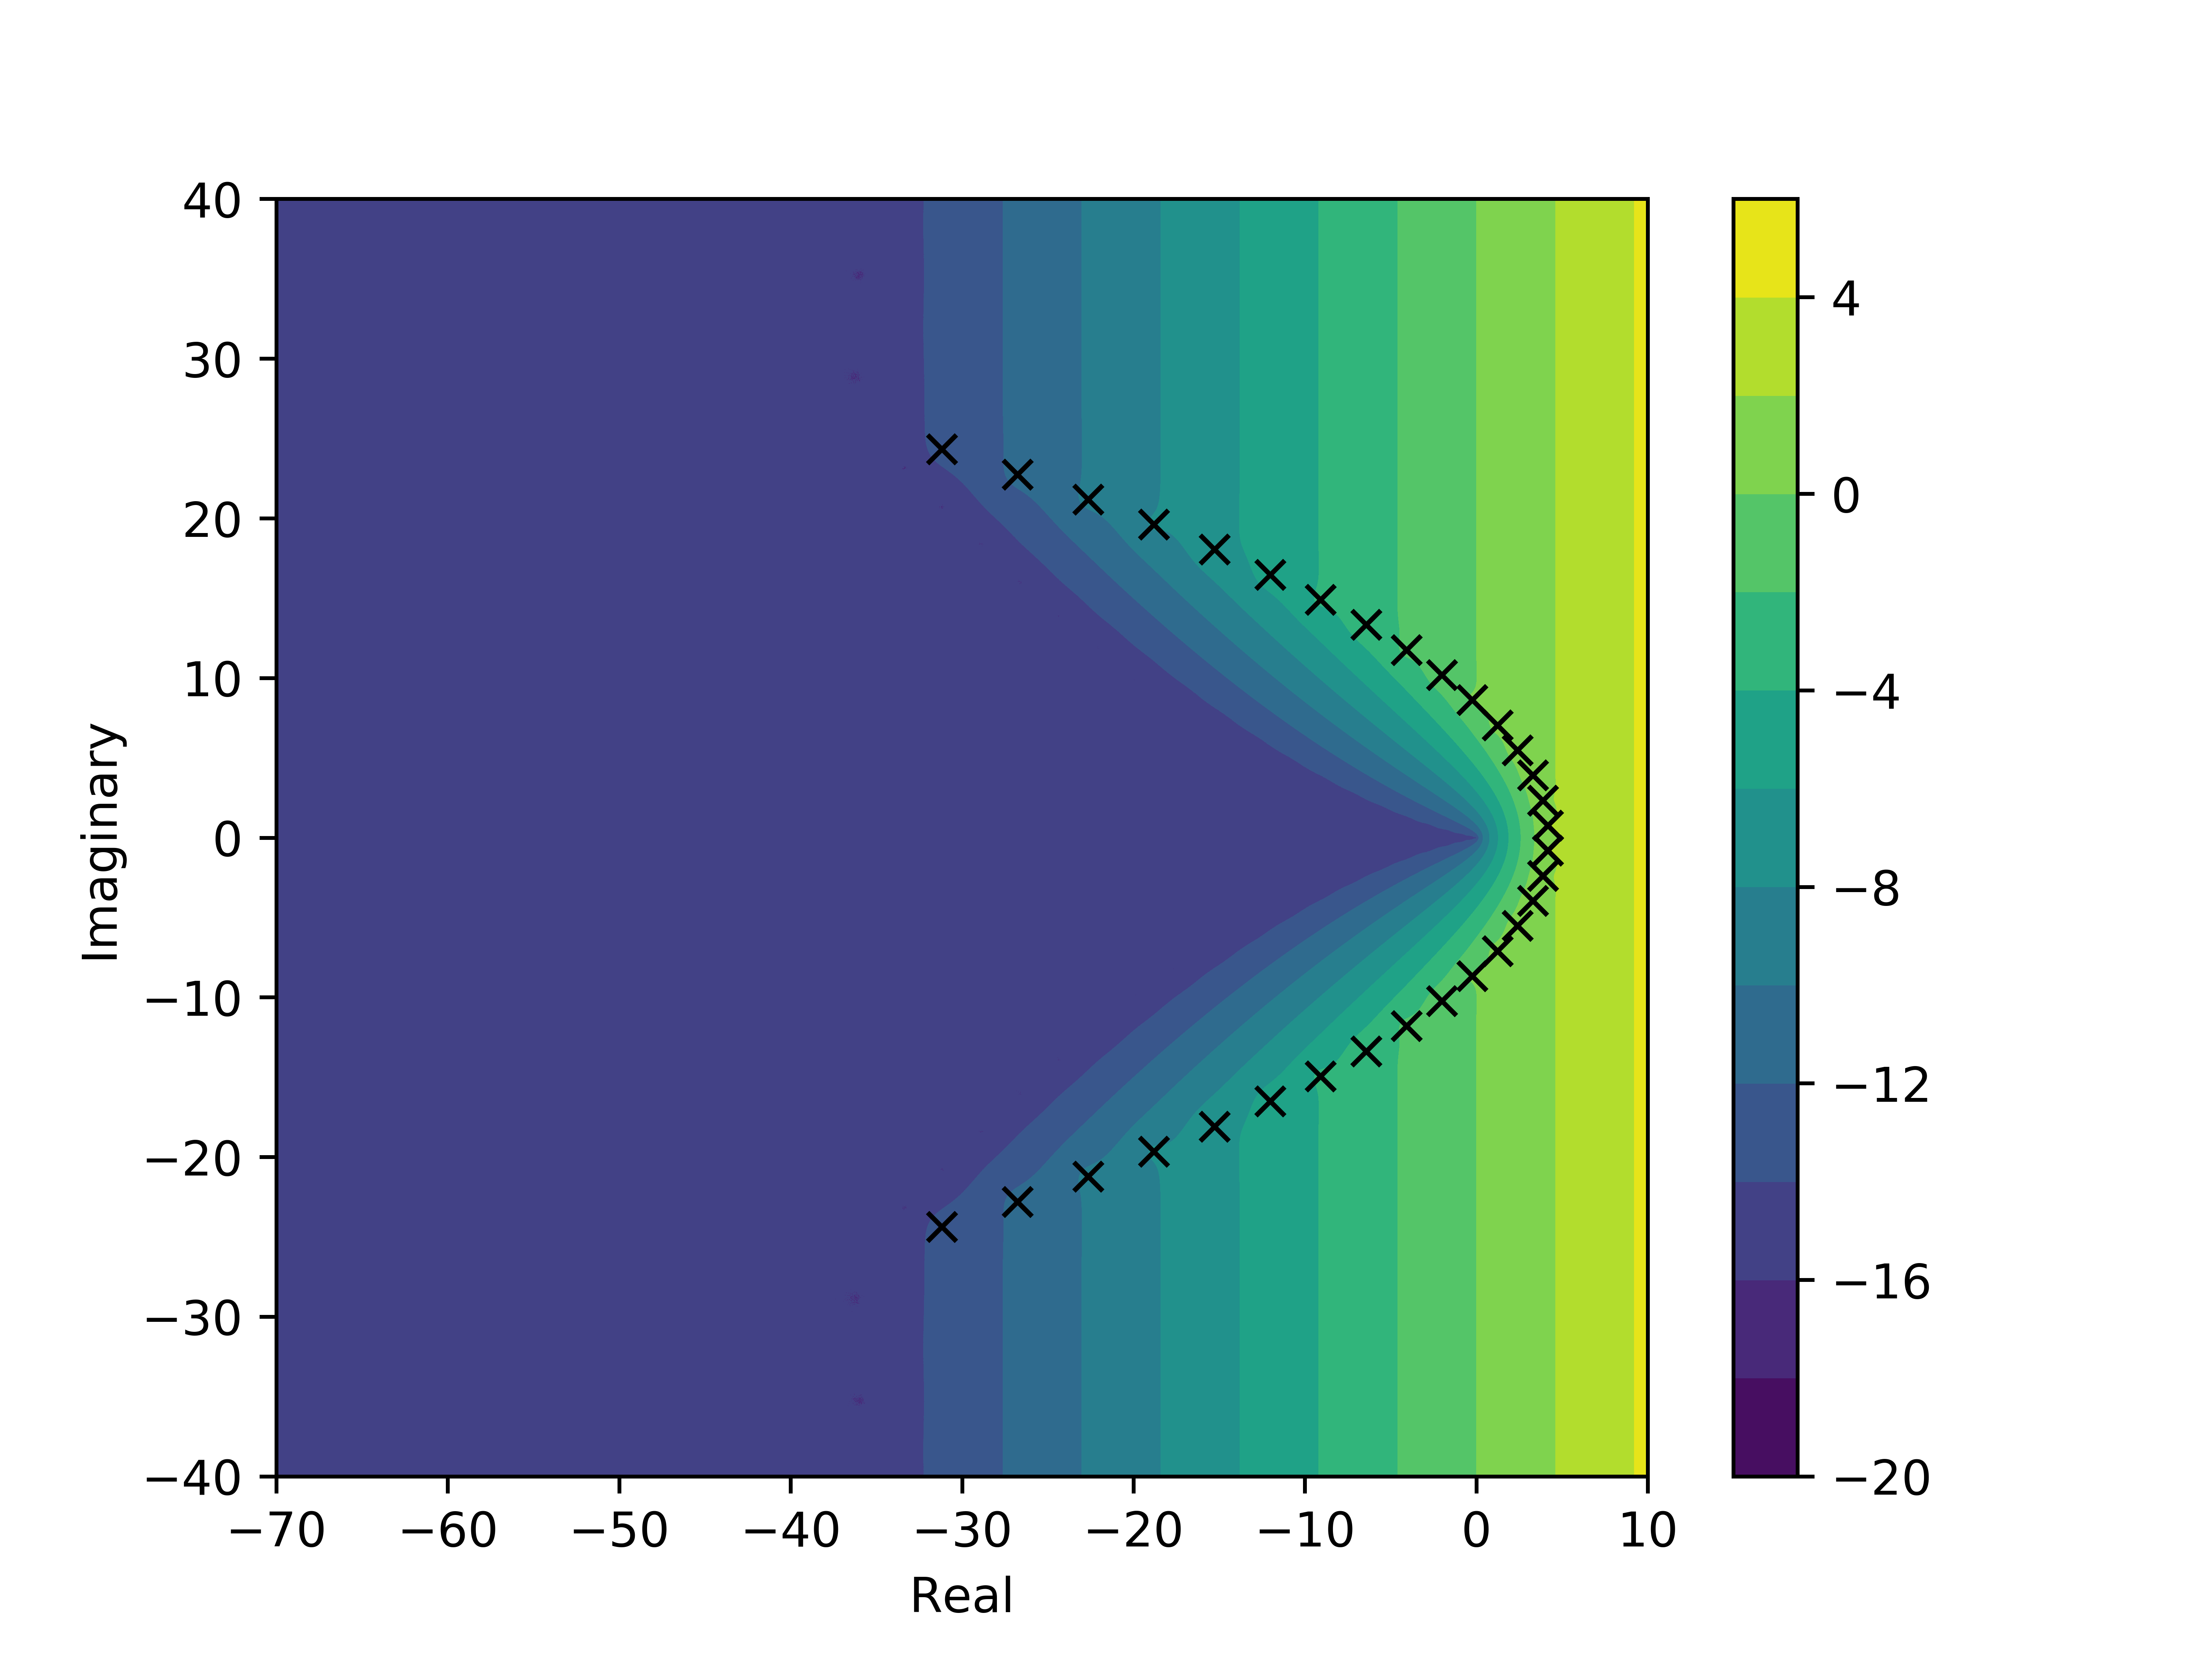
\includegraphics[width=5in]{images/chapter-3/RationApproxParabolicError32.png}\\
  \caption{$\log_{10}|r(z)-e^{z}|$ for N = 32 where the contour is defined by a parabola, Equation \ref{eq:parabolicContour}. Quadrature points are denoted with x's}
  \label{fig:complexRationalApproxParabola}
\end{figure} 

\clearpage

\begin{figure}[p]
  \centering
  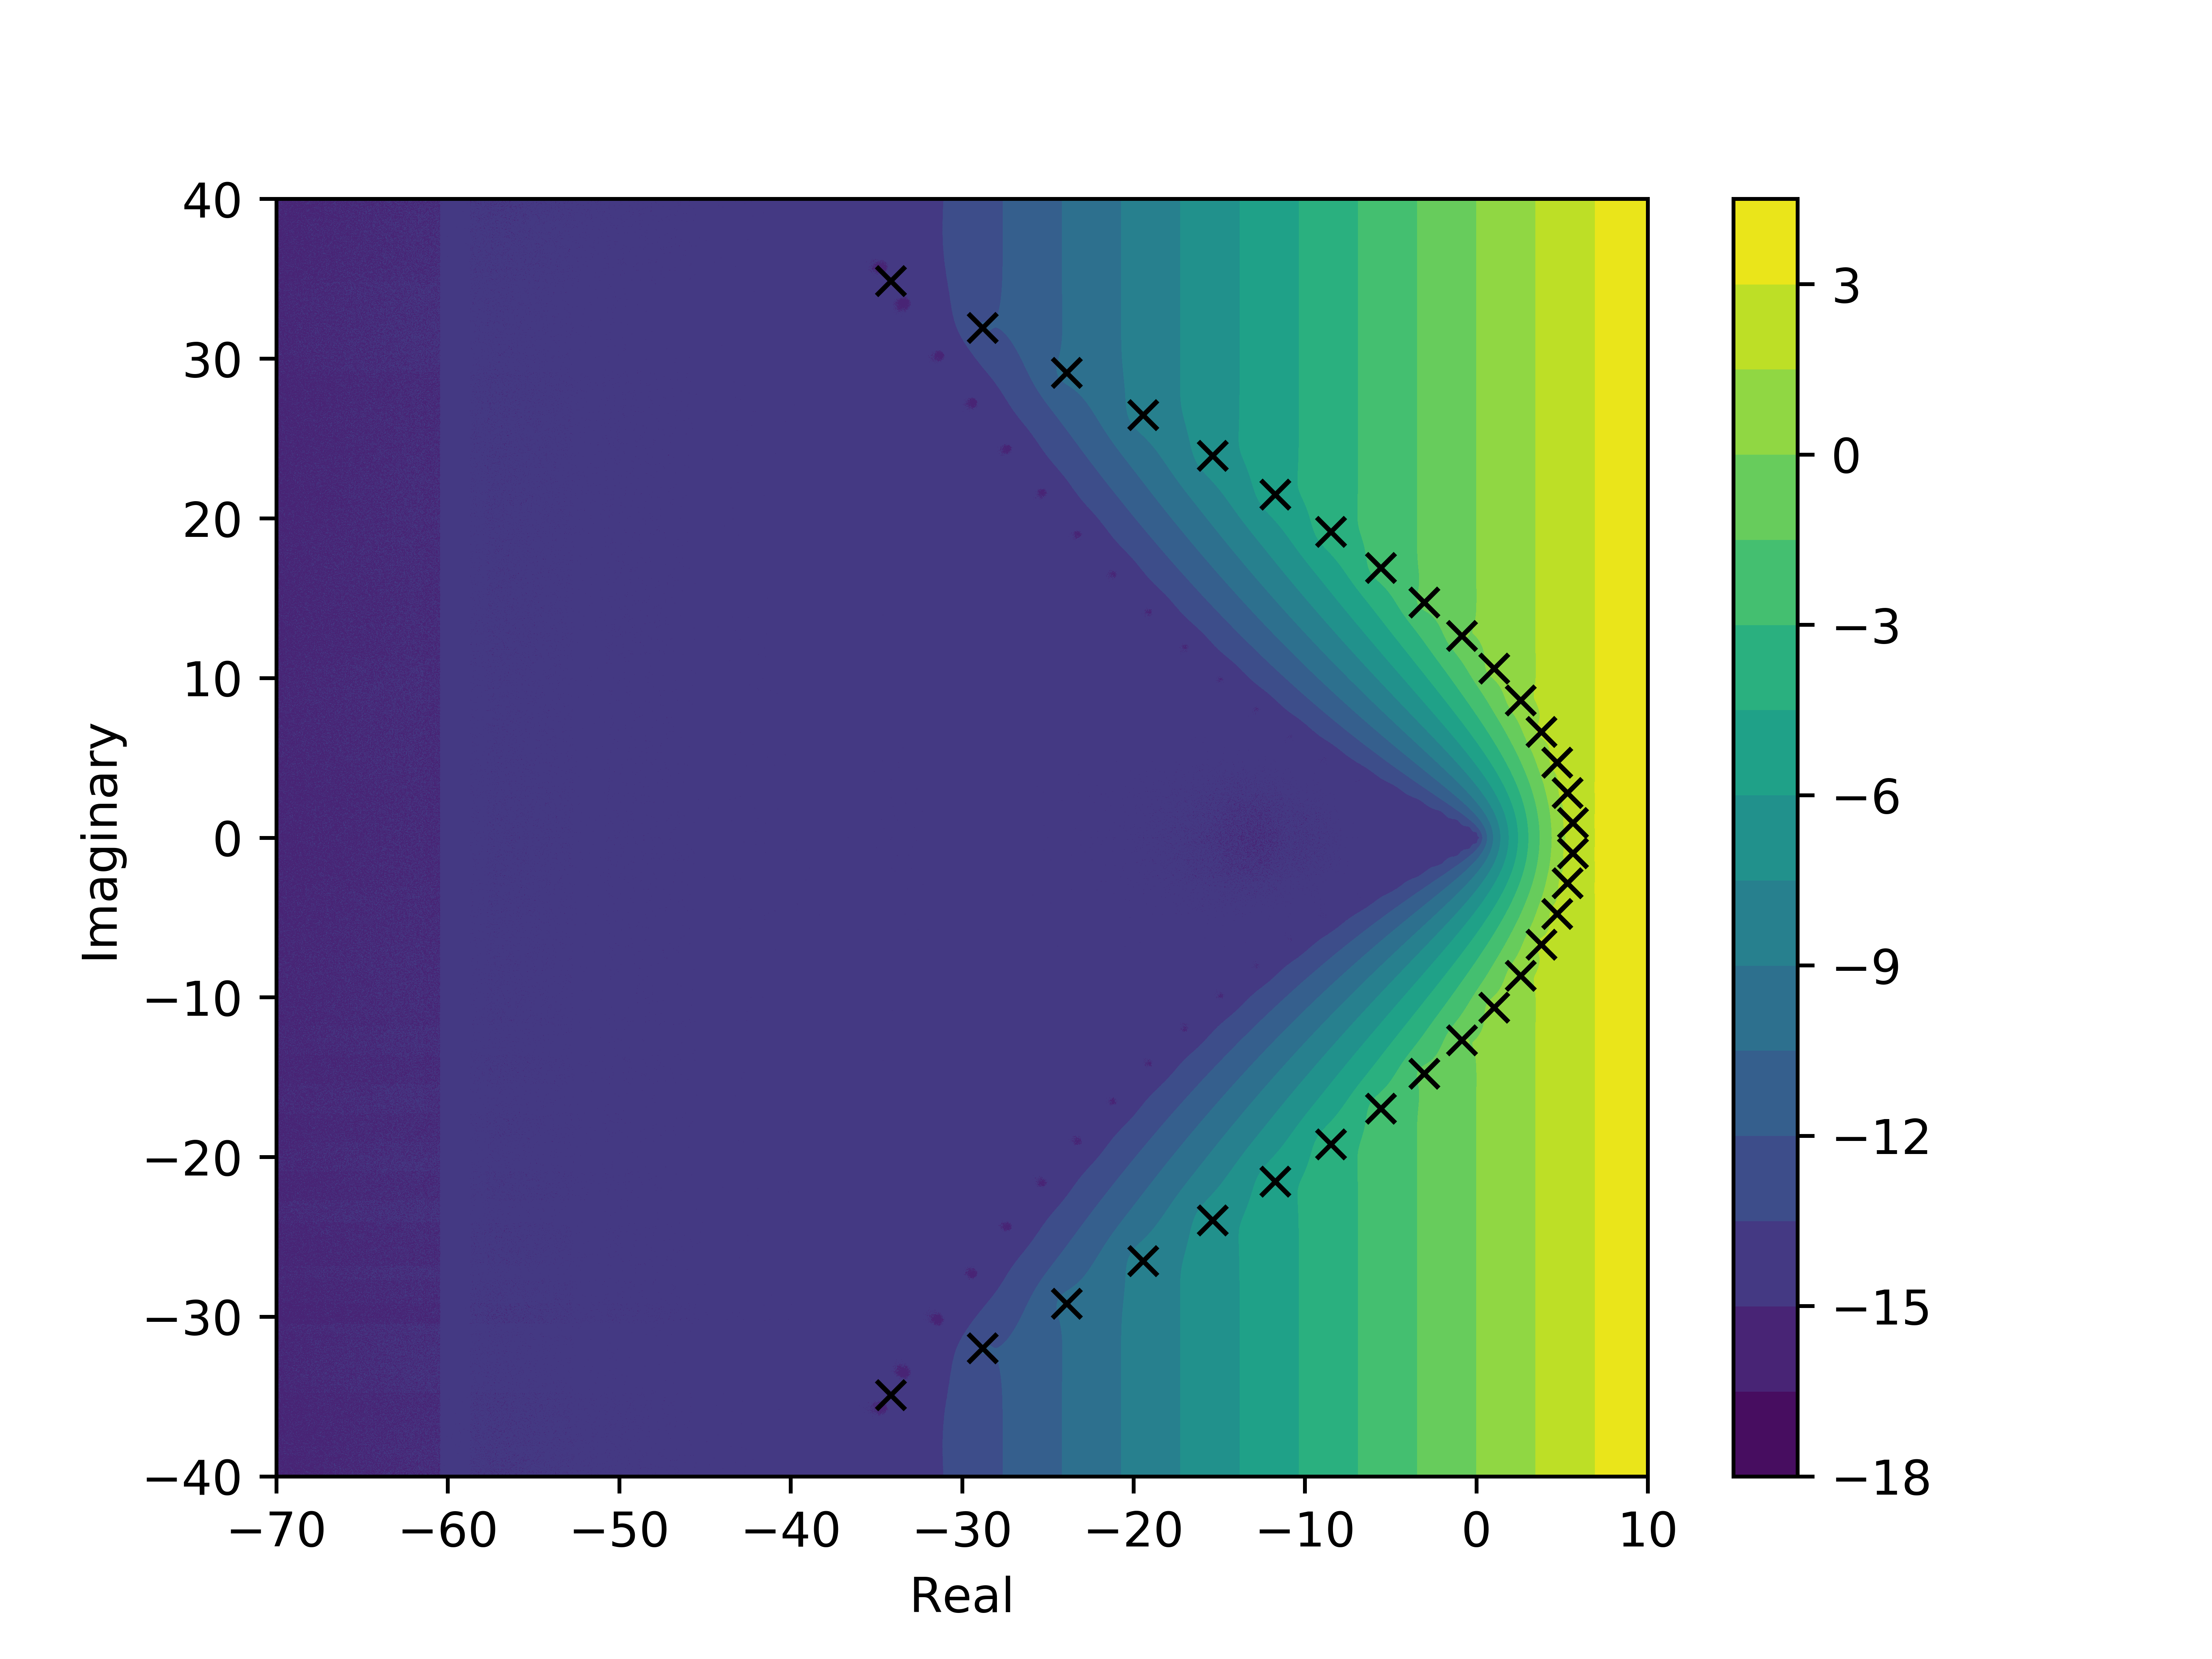
\includegraphics[width=5in]{images/chapter-3/RationApproxHyperbolicError32.png}\\
  \caption{$\log_{10}|r(z)-e^{z}|$ for N = 32 where the contour is defined by a hyperbola, Equation \ref{eq:hyperbolicContour}. Quadrature points are denoted with x's}
  \label{fig:complexRationalApproxHyperbola}
\end{figure} 

\clearpage

\noindent When applying the rational function to a real valued matrix, the approximation becomes,

\begin{equation}
    e^{\boldsymbol{A}} \approx r(\boldsymbol{A}) = 2Re\bigg(\sum_{k=1}^{N/2}c_{k}(\boldsymbol{A} - z_{k}\boldsymbol{I})^{-1}\bigg),
\end{equation}

\noindent requiring $N/2$ matrix inversions. If instead the action on the matrix exponential on a vector $\boldsymbol{v}$ is calculated, the approximation becomes,

\begin{equation}
    e^{\boldsymbol{A}}\boldsymbol{v} \approx r(\boldsymbol{A})\boldsymbol{v} = 2Re\bigg(\sum_{k=1}^{N/2}c_{k}(\boldsymbol{A} - z_{k}\boldsymbol{I})^{-1}\boldsymbol{v}\bigg),
\end{equation}

\noindent requiring $N/2$ solves of the linear system $\boldsymbol{x} = (\boldsymbol{A} - z_{k}\boldsymbol{I})^{-1}c_{k}\boldsymbol{v}$. It is important to note that each of these linear systems or matrix inversions are independent of one another and can be done in parallel. 

\subsubsection{Best Approximations}
A different approach is to choose a function $r(z)$ that is the best approximation of the exponential function on the negative real axis, doing this bypasses the need for a contour function \cite{pusaThesis} \cite{Trefethen2006}. This method is known as the Chebyshev Rational Approximation Method (CRAM) and is done by finding a unique rational function $\hat{r}_{k,k} = \hat{p}_{k}(x)/\hat{q}_{k}(x)$ satisfying 

\begin{equation}
    \epsilon_{k,k} \equiv \sup_{x \in \mathbb{R}_{-}} |\hat{r}_{k,k}(x) - e^{x}| = \inf_{r_{k,k} \in \pi_{k,k}}\bigg\{ \sup_{x \in \mathbb{R}_{-}} |r_{k,k}(x) - e^{x}|\bigg\}.
\end{equation}

\noindent Applying this definition leads to the following form on the rational approximation,

\begin{equation}
    e^{z} \approx r(z) = c_{0} + \sum_{k=1}^{N}\frac{c_{k}}{z - z_{k}}
\end{equation}


\noindent where $c_{0}$ is the limit at infinity. This formation is the same as the rational approximation with $c_{0} = 0$. The convergence rate for CRAM is of the order $\mathcal{O}(9.28903^{-N} )$, which is remarkably faster than those previously shown. With $N=16$ quadrature points CRAM gives about 15 or more digits of accuracy. Thus the same order of accuracy can be achieved with half the number of quadrature points than the rational approximations defined by contour functions. For a more detailed explanation the CRAM algorithm please refer to Reference \cite{pusaThesis}. 

The difficulty with using the CRAM approximation is finding the coefficient for the rational approximation. For CRAM of order 14 and 16 the rational coefficient can be found in Reference \cite{pusa2011} up to 20 digits. Figure \ref{fig:complexRationalApproxCRAM} shows the accuracy of CRAM to the function $e^{z}$ on the complex plane. Because the rational function was built in such a way to be the best approximation on the negative real axis, the accuracy of CRAM is in a more narrow range of the real axis. For a real values matrix the CRAM algorithm leads to the following solution,



\begin{equation}
    e^{\boldsymbol{A}} \approx r(\boldsymbol{A}) = c_{0} + 2Re\Bigg( \sum_{k=1}^{N/2}c_{k}(\boldsymbol{A} - z_{k}\boldsymbol{I})^{-1}\Bigg), 
\end{equation}

\noindent and for the action of the matrix on a vector,

\begin{equation}
    e^{\boldsymbol{A}}\boldsymbol{v} \approx r(\boldsymbol{A})\boldsymbol{v} = c_{0}\boldsymbol{v} + 2Re\Bigg( \sum_{k=1}^{N/2}c_{k}(\boldsymbol{A}t - z_{k}\boldsymbol{I})^{-1}\boldsymbol{v}\Bigg).
    \label{eq:CRAMVector}
\end{equation}

\subsubsection{Accuracy of Rational Approximations}
While the matrix exponential can be formally defined by Eq. (\ref{eq:power_series_exp}), when examining the accuracy of rational approximations presented, it is more useful to define the matrix exponential in terms of the transition matrix's eigenvalues. Because the contour $\Gamma$ must wind around the eigenvalues of $\boldsymbol{A}t$, if $\boldsymbol{A}$ has eigenvalues which have non-trivial imaginary parts then these eigenvalues will scale as a function of $t$. If these eigenvalues scale to a portion of the complex plane which fall outside the contour, then the accuracy of these methods can be compromised. For traditional burnup matrices it was stated earlier that the eigenvalues are clustered around the negative real axis \cite{pusa2010}. Because of this, the accuracy of CRAM as well as the other two rational approximations are not a function of time $t$ \cite{pusaAccruacy2013}. For burnup calculations in MSRs defined by Eq. (\ref{eq:MSRDepletion}) the eigenvalues are not necessarily clustered around the negative real axis as they have non-trival imaginary parts. Through numerical 

\clearpage

\begin{figure}[p]
  \centering
  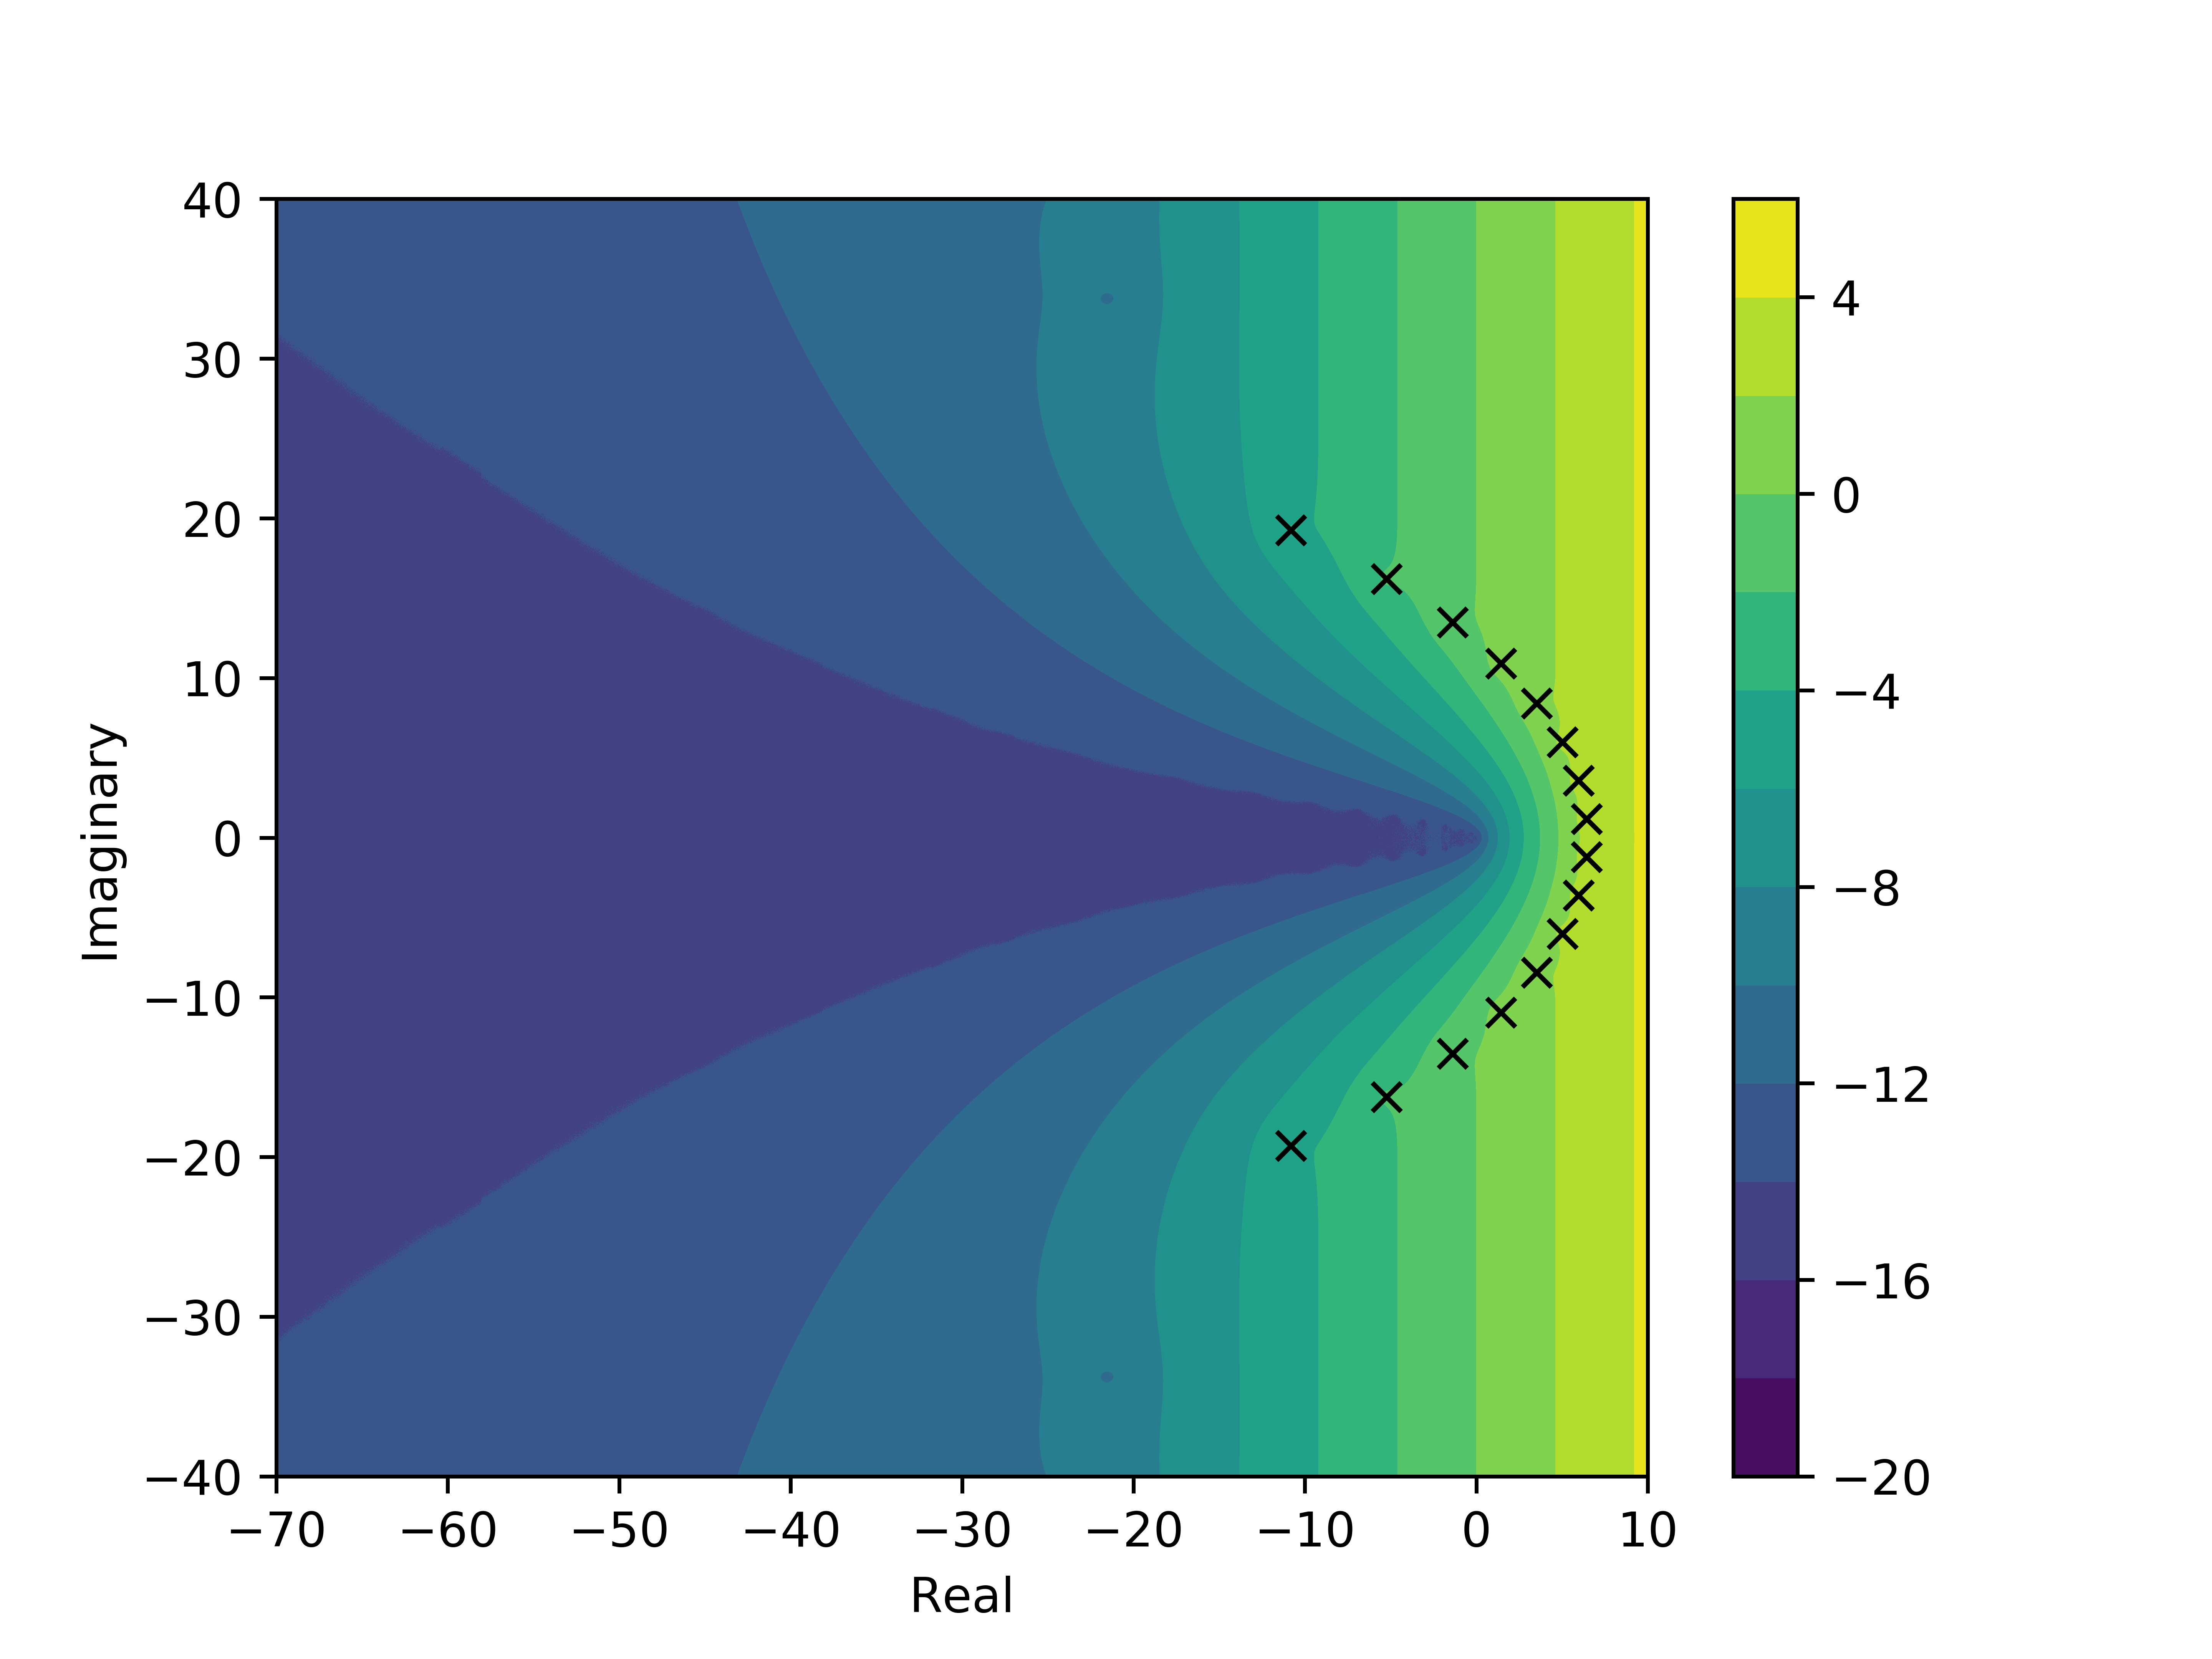
\includegraphics[width=5in]{images/chapter-3/RationApproxCRAMError16.png}\\
  \caption{$\log_{10}|r(z)-e^{z}|$ for CRAM with N = 16. Quadrature points are denoted with x's}
  \label{fig:complexRationalApproxCRAM}
\end{figure} 

\clearpage

\noindent experiments it was found by the author that these imaginary parts were introduced by the addition of convection terms in the transition matrix. In addition, these imaginary parts were found to be correlated with the ratio the velocity to the spatial discretization as well as the boundary conditions. 

While rational approximations such as CRAM have shown fantastic results in burnup calculations, is has been shown that the relative accuracy of CRAM diminishes when the nuclide concentration diminishes significantly over the time step. For a nuclide concentration $n_{i}(t) << n_{i}(0)$ the error estimate for CRAM follows \cite{isotalo2016}:

\begin{equation}
    \frac{\delta \hat{n}_{i}(t)}{n_{i}(t)} = \hat{\varepsilon}_{k,k} \frac{n_{i}(0)}{n_{i}(t)}
    \label{eq:CRAMError}
\end{equation}

\noindent This means that for CRAM of order $k$ concentration smaller than $\hat{\varepsilon}_{k,k}n_{i}(0)$ is not captured by the rational approximation. Additionally the accuracy of CRAM is diminished when performing calculations on fresh fuel versus depleted fuel. For fresh fuel, the concentrations of nuclides is dependent on transitions corresponding the only a few nuclides in the initial condition. If CRAM introduces large errors in approximating the matrix elements of a few transitions which influence the production of a large number of nuclides then the relative error in calculating nuclides concentrations diminishes. For used fuel depletion these errors are averaged out to provide an overall more accurate calculation. While this error was derived for transitional matrices built from solving tradition burnup calculations Eq. (\ref{eq:burnup}) it is assumed that the same holds true for MSR calculations of the form Eq. (\ref{eq:MSRDepletion}). In order to increase the accuracy of CRAM methods for depletion calculations a substepping approach was taken and introduced into the ORIGEN library \cite{isotalo2016}. This substepping method is also utilized in our implementation of the CRAM algorithm. 

It is important to note that the absolute error in computing rational approximations of the from parabolic or hyperbolic contours do not follow the same error as CRAM. In the scalar case of CRAM, if one plots the absolute error on the negative real axis as $x \rightarrow -\infty$, absolute error asymptotically approaches $\hat{\varepsilon}_{k,k}$. This is because the exponential function tends to zero while CRAM stabilizes at $\hat{\varepsilon}_{k,k}$. As $x \rightarrow 0$ the absolute error oscillates between $-\hat{\varepsilon}_{k,k}$ and $\hat{\varepsilon}_{k,k}$ \cite{pusaAccruacy2013}. While the errors for rational functions based on quadrature contours do not necessarily follow this same behavior, the substepping method was implemented and is later shown to also increase their accuracy. 

Substepping is implemented by scaling the time step size and evaluate the solution from the previous step, shown in Algorithm \ref{alg:substep}, where $m$ is the number of substeps to be taken. 

\begin{algorithm}
	\caption{Substeping} 
	\begin{algorithmic}[1]
	    \State $\boldsymbol{v}_{0} = \boldsymbol{\rho}_{0}$
	    \State $t = t/(m+1)$
		\For {$j=0,1,\ldots m$}
            \State $\boldsymbol{\rho}_{m+1} = r(\boldsymbol{A}t)\boldsymbol{v}_{0}$
            \State $\boldsymbol{v}_{0} = \boldsymbol{\rho}_{m+1}$
		\EndFor
	\end{algorithmic} 
	\label{alg:substep}
\end{algorithm}


\subsection{Krylov Subspace Method}
Krylov subpace approximations are a class of popular methods utilized in sparse matrix algorithms. The idea of Krylov subspace methods is to project the sparse $n \times n$ $\boldsymbol{A}$ matrix into a lower-dimensional subspace. The new lower dimension projection is of size $m \times m$ where $m < n$. Because the matrix is of lower dimension, calculating its matrix exponential becomes much faster. It is important to note that Krylov subspace methods can only be used as an operation on a vector, the direct calculation of the matrix exponential is not possible \cite{saad1992}.  

Consider we want to approximate the matrix exponential as a polynomial of order $m-1$, this takes the form,

\begin{equation}
    e^{\boldsymbol{A}}\boldsymbol{v} \approx p_{m-1}(A)\boldsymbol{v}.
    \label{eq:expPolynomailForm}
\end{equation}

\noindent This approximation is an element of the Krylov subspace defined by,

\begin{equation}
    K_{m} = \text{span}\{\boldsymbol{v}, \boldsymbol{A}\boldsymbol{v}, \boldsymbol{A}^{2}\boldsymbol{v}, ... ,\boldsymbol{A}^{m-1}\boldsymbol{v}\}.
\end{equation}

\noindent For a general non-symmetric matrix the Arnoldi algorithm can be utilized in building the Krylov space \cite{saad1992} \cite{saad1989}. Algorithm \ref{alg:arnoldi} constructs an orthonormal bases $\boldsymbol{V}_{m} = [\boldsymbol{v}_{1}, \boldsymbol{v}_{2}, ... \boldsymbol{v}_{m}]$ of the Krylov subspace, and an $m \times m$ upper Hessenberg matrix. The Arnoldi algorithm produces the following relation,

\begin{equation}
    \boldsymbol{A}\boldsymbol{V}_{m} = \boldsymbol{V}_{m}\boldsymbol{H}_{m} + h_{m+1,m}\boldsymbol{v}_{m+1}\boldsymbol{e}^{T}_{m}
    \label{eq:arnoldiResult}
\end{equation}

\begin{algorithm}
	\caption{Arnoldi} 
	\begin{algorithmic}[1]
	    \State Compute $\boldsymbol{v}_{1} = \boldsymbol{v}/||\boldsymbol{v}||_{2}$
		\For {$j=1,2,\ldots m$}
            \State Compute $\boldsymbol{w} = \boldsymbol{A}\boldsymbol{v}_{j}$
            \For{$i=1,2,\ldots j$}
                \State Compute $h_{i,j} = (\boldsymbol{w},\boldsymbol{v}_{i})$
                \State Compute $\boldsymbol{w} = \boldsymbol{w} - h_{i,j}\boldsymbol{v}_{i}$
            \EndFor
            \State Compute $h_{j+1, j} = ||\boldsymbol{w}||_{2}$ and $\boldsymbol{v}_{j+1} = \boldsymbol{w}/h_{j+1,j}$
		\EndFor
	\end{algorithmic} 
	\label{alg:arnoldi}
\end{algorithm}

\noindent where $\boldsymbol{H}_{m} = \boldsymbol{V}^{T}_{m}\boldsymbol{A}\boldsymbol{V}_{m}$ and $\boldsymbol{e}_{m}$ is the unit vector of dimension $m$. The Hessenberg matrix $\boldsymbol{H}_{m}$ represents the projection of $\boldsymbol{A}$ on to the Krylov subspace. The approximation in Krylov space is known to be, 

\begin{equation}
    e^{\boldsymbol{A}}\boldsymbol{v} \approx \beta \boldsymbol{V}_{m}e^{\boldsymbol{H}_{m}}\boldsymbol{e}_{1}
    \label{eq:krylovApproxEXP}
\end{equation}

\noindent where $\beta = ||\boldsymbol{v}||_{2}$ \cite{saad1989}. The computation of $e^{
\boldsymbol{H}_{m}}$ becomes much easier because $\boldsymbol{H}_{m}$ is dense and smaller than $\boldsymbol{A}$. After the Krylov approximation is made, a typical method for solving the matrix exponential is used on $e^{\boldsymbol{H}_{m}}$. The quality of this approximation is exact when $n = m$. This comes from the fact that at step $m$, $h_{m+1,m} = 0$ and Equation \ref{eq:arnoldiResult} becomes,

\begin{equation}
    \boldsymbol{A}\boldsymbol{V}_{m} = \boldsymbol{V}_{m}\boldsymbol{H}_{m}.
\end{equation}

\noindent The Arnoldi process will be exact after $m$ steps when $m$ is greater to or equal to the degree of the minimal polynomial in Equation \ref{eq:expPolynomailForm}. At this point Equation \ref{eq:expPolynomailForm} is exact, however this is unlikely to happen until $m=n$ \cite{saad1992} \cite{saad1989}. 

 The general error associated with applying the approximation in Equation \ref{eq:krylovApproxEXP} can be proven to be,
 
 \begin{equation}
     ||e^{\boldsymbol{A}}\boldsymbol{v} - \beta \boldsymbol{V}_{m}e^{\boldsymbol{H}_{m}}\boldsymbol{e}_{1}||_{2} \leq 2\beta \frac{\rho^{m}e^{\rho}}{m!},
 \end{equation}
 
 \noindent where $\rho = ||A||_{2}$ \cite{saad1992}. The error bounds derived by Saad in \cite{saad1992} can be computed but might not be sharp, especially when the norm of the matrix is large. In practice, a more useful posteriori error can be used to determine the error for applying the Arnoldi algorithm. This error is found after applying the Arnoldi algorithm and is defined by,
 
\begin{equation}
    ||e^{\boldsymbol{A}}\boldsymbol{v} - \beta \boldsymbol{V}_{m}e^{\boldsymbol{H}_{m}}\boldsymbol{e}_{1}||_{2} \approx h_{m+1,m}|\boldsymbol{e}_{m}^{T}\phi(\boldsymbol{H}_{m})\beta \boldsymbol{e}_{1}|,
\end{equation}

\noindent where $\phi(\boldsymbol{A}) = \boldsymbol{A}^{-1}[e^{\boldsymbol{A}} - \boldsymbol{I}]$. This error estimate was found to be sufficient enough for practical applications \cite{saad1992}. 

Krylov subpsace methods are good for approximating the largest eigenvalues of a matrix because of the continued multiplication of $\boldsymbol{A}$ when computing the orthonormal basis \cite{akio2007}. As the spread of the eigenvalues for $\boldsymbol{A}$ increases the accuracy of the Krylove subspace decreases, even as you increase the dimension of the subspace \cite{pusa2010}. 